\chapter{Spending less per trial: multi-fidelity methods}
\label{sec:multifidelity}

Everything in Chapter~\ref{sec:bayesian} treats a trial as atomic: pick a
configuration, pay full price, observe the final score. But training
produces a stream of intermediate evidence, and most bad configurations
announce themselves early. In the running example, a learning rate of
$10^{-2}$ that sends PPO's policy loss to infinity does so within the first
million environment steps; paying for the remaining 149 million to confirm
the diagnosis is charity. Methods that act on partial evaluations are
called multi-fidelity methods, and they are the largest single source of
savings available to us.

The catch, which every method in this chapter manages in its own way, is
that low-fidelity performance is only a proxy, and the proxy is biased in a
known direction: rankings at epoch five need not match rankings at epoch
fifty, and the disagreement is not symmetric noise. Small learning rates
and heavy regularization look bad early and win late; aggressive settings
sprint and stall. Figure~\ref{fig:curves} draws the failure we must
design against: at the first checkpoint the eventual winner is in last
place, so a scheduler that culls hard on early evidence systematically
kills slow starters. Whether early rankings can be trusted is an empirical
property of each workload, worth a pilot measurement (a rank correlation
between fidelities on a handful of configurations) before committing to an
aggressive schedule.

\begin{figure}[t]
\centering
\begin{tikzpicture}[scale=1.0, font=\small]
\draw[-{Latex}] (0,0) -- (9.3,0);
\node[anchor=north] at (7.6,-0.6) {training budget (fidelity)};
\draw[-{Latex}] (0,0) -- (0,4.3);
\node[rotate=90, anchor=south] at (-0.4,2.15) {evaluation score};
% rung lines
\foreach \x/\l in {1.5/rung 1, 4.5/rung 2, 8.6/rung 3}
  \draw[dotted] (\x,0) node[below, font=\footnotesize] {\l} -- (\x,4.1);
% fast starter that stalls
\draw[thick, red!60!black, densely dashed]
  (0,0.2) .. controls (0.7,1.7) and (1.2,2.3) .. (1.5,2.5)
  .. controls (2.6,3.0) and (3.6,3.1) .. (4.5,3.1)
  .. controls (5.8,3.1) and (7.2,3.05) .. (8.6,3.0);
\node[red!60!black, anchor=west] at (6.55,2.7) {sprints, then stalls};
% slow starter that wins
\draw[thick, blue!60!black]
  (0,0.1) .. controls (0.9,0.5) and (1.2,0.7) .. (1.5,0.9)
  .. controls (2.6,1.7) and (3.6,2.5) .. (4.5,3.0)
  .. controls (5.8,3.6) and (7.2,3.9) .. (8.6,4.0);
\node[blue!60!black, anchor=west] at (5.3,4.05) {slow starter, eventual winner};
% cull marker at rung 1
\draw[-{Latex}, thick] (1.9,0.35) -- (1.58,0.82);
\node[anchor=west, align=left] at (1.9,0.32) {culled here if rung 1 cuts too hard};
\end{tikzpicture}
\caption{The multi-fidelity hazard (schematic). At rung 1 (the first of
the budget checkpoints that this chapter's ladders call rungs) the aggressive
configuration leads and the eventual winner trails; their curves cross
between rungs 1 and 2. Every method in this chapter is a different answer
to the question ``how hard may we cut on early evidence, given that curves
cross?'', and the honest answer starts with measuring how often they cross
on the workload at hand.}
\label{fig:curves}
\end{figure}

\section{Successive halving: the arithmetic of courage}

Successive halving spends a budget on many cheap looks and a few expensive
ones \citep{jamieson2016successive}. Fix a reduction factor $\eta$
(usually 3). Give every starter a small budget $r$; keep the best $1/\eta$
fraction and give each survivor $\eta$ times more budget; repeat. The
rounds of this ladder are called \emph{rungs}, and the race ends when
one rung remains. Rung sizes shrink by $\eta$ while per-trial budgets grow by
$\eta$, so every rung costs about the same, and there are about
$\log_\eta n$ rungs of them.

The numbers deserve one concrete pass, because the savings are the whole
argument. Take the running example with $n = 81$ starting configurations,
$\eta = 3$, and an initial budget of $r$ = 1 unit, where 81 units is a
full training run (so one unit is just under two million environment
steps). The rungs then look like this:
81 trials at 1 unit each (cost 81), the best 27 continue to 3 units
(cost 81), the best 9 continue to 9 units (cost 81), the best 3 continue
to 27 units (cost 81), and the single survivor runs to the full 81 units
(cost 81). Total: 405 units, about five full-length runs, to triage 81
configurations. Evaluating all 81 at full length would have cost
$81 \times 81 = 6561$ units, a factor of sixteen more; even the standard
sixteen-full-runs budget of the RL study in
Chapter~\ref{sec:workloads} could not have screened a fifth as many
candidates at full fidelity. Figure~\ref{fig:sh} draws the resulting
shape: the budget is a rectangle of constant area per rung, spent mostly
on configurations that survived at least one cut.

\begin{figure}[t]
\centering
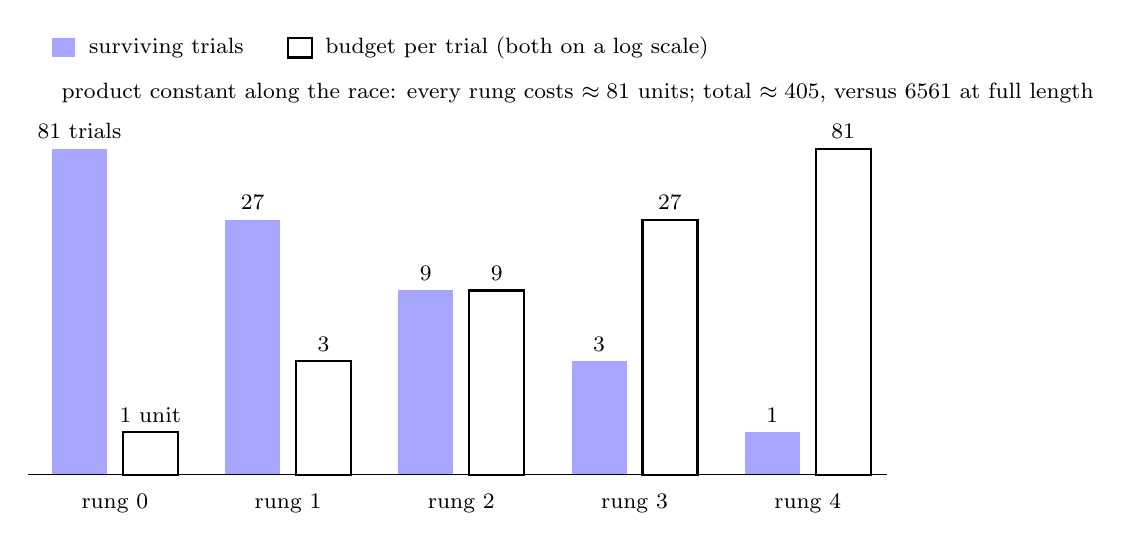
\begin{tikzpicture}[font=\small]
% paired bars per rung: filled = surviving trials, open = per-trial budget (log scale)
\foreach \rung/\ha/\hc/\la/\lc in {0/4.14/0.54/81 trials/1 unit, 1/3.24/1.44/27/3, 2/2.34/2.34/9/9, 3/1.44/3.24/3/27, 4/0.54/4.14/1/81} {
  \fill[blue!35] (2.2*\rung,0) rectangle (2.2*\rung+0.7,\ha);
  \draw[thick] (2.2*\rung+0.9,0) rectangle (2.2*\rung+1.6,\hc);
  \node[anchor=south, font=\footnotesize] at (2.2*\rung+0.35,\ha) {\la};
  \node[anchor=south, font=\footnotesize] at (2.2*\rung+1.25,\hc) {\lc};
  \node[anchor=north, font=\footnotesize] at (2.2*\rung+0.8,-0.12) {rung \rung};
}
\draw (-0.3,0) -- (10.6,0);
% legend
\fill[blue!35] (0.0,5.3) rectangle (0.3,5.55);
\node[anchor=west, font=\footnotesize] at (0.35,5.42) {surviving trials};
\draw[thick] (3.0,5.3) rectangle (3.3,5.55);
\node[anchor=west, font=\footnotesize] at (3.35,5.42) {budget per trial (both on a log scale)};
\node[anchor=west, font=\footnotesize, align=left] at (0.0,4.85)
  {product constant along the race: every rung costs $\approx 81$ units; total $\approx 405$, versus $6561$ at full length};
\end{tikzpicture}
\caption{One successive-halving bracket on the running example
($n = 81$, $\eta = 3$). At each rung the surviving trials shrink by the
factor the per-trial budget grows by, so the two staircases mirror each
other and every rung costs the same 81 units: the whole screen of 81
configurations costs about five full-length runs. The scheme's entire
risk is concentrated in the cuts between rungs, where
Figure~\ref{fig:curves}'s crossing curves get judged early.}
\label{fig:sh}
\end{figure}

The rub is the choice of the starting budget $r$: too small and slow
starters die unfairly (the hazard of Figure~\ref{fig:curves} at its
sharpest), too large and the savings evaporate. Hyperband declines to
choose. It runs several successive-halving brackets, from aggressive
(many configurations, tiny initial budget) to conservative (few
configurations, nearly full initial budget), giving each bracket the
same total budget, and provably loses only a logarithmic factor to the
best bracket in hindsight \citep{li2018hyperband}. Continuing the
numbers above ($\eta = 3$, full budget 81 units), the five brackets
start 81 trials at 1 unit, 34 at 3, 15 at 9, 8 at 27, and 5 at the full
81, each bracket then halving as before; each costs about 405 units, so
the whole portfolio costs about 2025 units, twenty-five full-run
equivalents to hedge every plausible answer to ``how early is too early
to judge.'' On a workload where early rankings are honest, the
aggressive brackets deliver; on one where curves cross late, the
conservative brackets are the insurance policy that was bought in
advance.

\section{The asynchronous turn}

Both methods as stated are synchronous: a rung must fully finish before
promotions happen, so a single straggler idles the fleet. With hundreds
of workers this is not a corner case; it is the steady state.

ASHA,
the asynchronous successive halving algorithm,
removes the barrier \citep{li2020asha}. Whenever a worker frees up, look
at the topmost rung that has a promotable trial: promote any
configuration that is in the top $1/\eta$ of the results recorded so far
at its rung; otherwise start a fresh configuration at the bottom rung.
Concretely: with $\eta = 3$, the moment the fourth result lands on a
rung, its best member is in the top third of four and can be promoted
immediately, without waiting for trials five through eighty-one.

Early
promotions are sometimes wrong (judged against a rung that was not full
yet), and ASHA accepts this deliberately: the authors' experiments show
the aggressiveness costs little in final quality while keeping hundreds
of workers busy, and ASHA has become the standard early-stopping
scheduler in distributed tuners, including Ray Tune's implementation.
The design lesson generalizes and will return in
Chapter~\ref{sec:population}: at scale, a slightly worse decision now
beats a slightly better decision after a barrier.

Two refinements are worth knowing. PASHA grows the maximum fidelity
progressively and stops growing it once the ranking of survivors
stabilizes, saving the top-rung budget when the decision is already
clear \citep{bohdal2023pasha}. The median stopping rule, older and
model-free, simply kills any trial whose running average falls below the
median of completed trials at the same step \citep{golovin2017vizier};
it composes with any searcher and is the cheapest insurance policy we
can offer users.

\section{Putting the model back: BOHB, DEHB, and racing}

Bandit schedulers decide when to stop but sample new configurations
blindly: the bottom rung of every bracket above was filled by random
search. After Chapter~\ref{sec:bayesian}, the obvious repair is to let a
model choose what enters the race. BOHB, Bayesian optimization plus
Hyperband as its name says, runs Hyperband's brackets but
draws new configurations from a TPE fit at the highest fidelity that has
enough observations, so the racing machinery keeps its budget arithmetic
while the entrants improve over time \citep{falkner2018bohb}. DEHB
replaces the sampler with differential evolution
(Chapter~\ref{sec:modelfree}): a subpopulation evolves at each rung, and
information flows across fidelities through the evolutionary operations
themselves, survivors of cheap rungs seeding the recombination that
proposes candidates for expensive ones, rather than through a fitted
density model \citep{awad2021dehb}.

DEHB deserves particular attention from us: in the controlled comparison
of \citet{eimer2023hyperparameters} across PPO and two other standard
RL algorithms (SAC and DQN) on eleven
environments, DEHB was the most consistent tuner at budgets of ten to
sixty-four full training runs, matching or beating hand tuning, random
search, and the population methods, all at negligible optimizer
overhead. That is precisely the budget regime our routine RL studies
live in, and Chapter~\ref{sec:workloads} builds the recommendation on
it. SMAC3 reaches a similar design point from the BO side, pairing its
random forest surrogate with successive-halving style racing of
incumbents \citep{lindauer2022smac3}.

\section{Modeling the learning curve itself}

Rung-based methods compare trials only at matching fidelities and throw
away the shape of the curve between rungs; in Figure~\ref{fig:curves},
the information that the blue curve was still rising steeply at rung 1
while the red curve had flattened is exactly what the rung comparison
discards. Learning-curve methods keep it. They model the whole
trajectory and ask a sharper question: given everything observed so far,
which paused trial (or which new one) should receive the next slice of
budget? Figure~\ref{fig:freezethaw} shows the decision problem: from a
partial curve, extrapolate a distribution over its continuation, and
weigh thawing the promising-but-uncertain run against extending the
solid-but-plateauing one.

\begin{figure}[t]
\centering
\begin{tikzpicture}[scale=1.0, font=\small]
\draw[-{Latex}] (0,0) -- (9.3,0);
\node[anchor=north] at (7.9,-0.12) {training budget};
\draw[-{Latex}] (0,0) -- (0,4.3);
\node[rotate=90, anchor=south] at (-0.4,2.15) {evaluation score};
\draw[dotted] (3.6,0) node[below, font=\footnotesize] {observed so far} -- (3.6,4.1);
% observed curve
\draw[thick, blue!60!black]
  (0,0.2) .. controls (1.2,1.2) and (2.4,2.0) .. (3.6,2.4);
% extrapolation fan
\fill[blue!12]
  (3.6,2.4) .. controls (5.2,3.4) and (7.0,3.9) .. (9.0,4.05)
  -- (9.0,2.2) .. controls (7.0,2.5) and (5.2,2.5) .. (3.6,2.4) -- cycle;
\draw[blue!60!black, densely dashed]
  (3.6,2.4) .. controls (5.2,3.0) and (7.0,3.2) .. (9.0,3.2);
\node[blue!60!black, anchor=west, align=left] at (6.4,4.15) {posterior over the continuation};
% competitor: paused flat curve
\draw[thick, red!60!black]
  (0,0.4) .. controls (1.2,1.9) and (2.4,2.6) .. (3.6,2.8);
\draw[red!60!black, densely dashed]
  (3.6,2.8) .. controls (5.2,3.0) and (7.0,3.05) .. (9.0,3.05);
\node[red!60!black, anchor=west] at (0.45,3.5) {leads today, extrapolation flat};
\draw[red!60!black, -{Latex}] (4.05,3.5) -- (5.3,3.08);
\node[blue!60!black, anchor=west, font=\footnotesize] at (1.75,0.5) {trails today, still rising};
\end{tikzpicture}
\caption{The freeze-thaw decision (schematic). Both trials are paused at
the dotted line. The red trial leads today but its extrapolation is
flat; the blue trial trails with a rising curve and a wide posterior
over where it ends up. A learning-curve method allocates the next budget
slice by comparing these posteriors, information that rung-based
promotion never sees.}
\label{fig:freezethaw}
\end{figure}

The idea goes back to freeze-thaw Bayesian optimization
\citep{swersky2014freezethaw}, which kept a basket of paused runs
(freeze a run to pause it, thaw it to resume) and
used a GP with an exponential-decay kernel over training curves to
decide which to thaw. Every modern instance keeps that decision
structure and changes one component, the curve model, and the choice
matters more than it sounds, because the curve model is refit inside
the decision loop: whatever it costs is paid again at every
allocation decision.

DyHPO makes the curve model a deep-kernel GP over the triple of
configuration, budget, and partial curve, and greedily advances
whichever candidate has the best expected improvement one step ahead
\citep{wistuba2022dyhpo}. The price follows from
Chapter~\ref{sec:bayesian}: GP fitting is cubic in the number of
observations, and a curve observed at every epoch multiplies
observations quickly, so the surrogate's bill grows with exactly the
data that makes it useful.

DPL swaps the GP for an ensemble of power-law extrapolations,
motivated by the empirical regularity that neural training curves
follow approximate power laws; the spread of the ensemble supplies
the uncertainty that the acquisition needs \citep{kadra2023dpl}. The
model is lighter than a deep-kernel GP, but the ensemble is still
refit inside the loop.

ifBO (in-context freeze-thaw BO) removes the in-loop fitting entirely.
Its curve model is a prior-fitted network: a transformer (the neural
architecture behind modern language models) pre-trained once on
synthetic learning curves, which then performs Bayesian curve
extrapolation
in-context, in a single forward pass, one to two orders of magnitude
faster than fitting DyHPO's deep GP or DPL's ensembles inside the
loop. The acquisition paired with it randomizes its lookahead horizon
and improvement threshold \citep{rakotoarison2024ifbo}.
Chapter~\ref{sec:transfer} explains what a prior-fitted network is
and why ``pre-trained once'' is the phrase that changes the
economics.

The evidence and the price, briefly, before the evidence section
weighs both. On the multi-fidelity benchmarks used in those papers,
the learning-curve methods dominate rung-based baselines when curves
are informative. The price is operational: the tuner must be able to
pause, checkpoint, and resume trials at fine granularity, which is
exactly the machinery that Ray Tune trials and RLlib checkpoints
already expose.

The honest summary for our roadmap: ASHA plus a good searcher is the
sturdy default that captures most of the savings; DEHB is the
evidence-backed choice at small RL budgets; learning-curve methods are
the frontier worth one focused implementation
(Chapter~\ref{sec:roadmap}) once the pause and resume plumbing is
solid, with ifBO the most attractive because the surrogate arrives
pre-trained rather than being refit inside the loop.

\section{The evidence, and how much of it is arithmetic}
\label{sec:mf-evidence}

Those verdicts lean on four different grades of support, and the
grades are worth keeping separate because each properly carries a
different weight of decision: arithmetic, which requires no trust in
anyone; theory, which is genuine but conditional; the method authors'
own benchmarks; and a single independent study on live training runs.
Section~\ref{sec:bo-evidence} argued that evidence should be weighed
by how it was produced. Applied here, that principle sorts the
chapter's claims cleanly.

The arithmetic came first, and it is the part that cannot be argued
with. The 405-versus-6561 comparison under Figure~\ref{fig:sh} is not
an experimental finding; given the rung geometry, the factor of
sixteen follows by multiplication, and no benchmark can add to it or
take it away. What multiplication cannot supply is a promise that the
cheap rungs \emph{select} well, and the theory is candid about the
same limit. The successive-halving guarantee is of a deliberately
modest kind, bounding identification error under assumptions on how
fast each training curve settles toward its final value, and
Hyperband's theorem promises performance within a logarithmic factor
of the best bracket in hindsight, not good performance outright
\citep{jamieson2016successive, li2018hyperband}. Neither theorem knows
whether the curves of our workloads settle quickly enough for early
rankings to be trusted. That is a property of the workload, not of
the algorithm, which is why the rank-correlation pilot suggested at
the chapter's opening is the one empirical measurement the whole
apparatus genuinely needs.

ASHA's evidence is of another kind again, and the paper it comes from
announces what kind: this is a systems paper, written around the
production tuning service its authors were building, and its central
claims are operational \citep{li2020asha}.

The distributed
experiments compare ASHA against synchronous successive halving,
BOHB, and PBT (the population method Chapter~\ref{sec:population}
teaches) with twenty-five workers on two image-classification tuning
tasks (CIFAR-10),
five runs of each method, and the finding is the one the mechanism
predicts: on the task where training times vary across
configurations, the synchronous methods idle at their barriers and
ASHA pulls cleanly ahead, while on the task where they do not, the
schedulers roughly agree, ASHA reaching a good configuration about
1.5 times sooner and BOHB ending slightly ahead on final quality. On
two architecture search spaces with sixteen workers, ASHA reached a
below-ten-percent test error roughly twice as fast as synchronous
halving and BOHB and ended slightly ahead on average. The
demonstration that justifies the word ``massive'' ran five hundred
workers for weeks on a recurrent language-model space.

All of this is the authors' own
arena, and the selection-bias caution of
Section~\ref{sec:bo-evidence} applies; two things temper it here.
The claim under test is throughput rather than statistical
cleverness, so a skeptic can audit the mechanism (promote now
against the top third observed so far, never wait) instead of
trusting a tuned baseline. And the operational half of the claim has
been replicated the way operational claims are: ASHA is the standard
early-stopping scheduler in the distributed tuners we audited
(Chapter~\ref{sec:libraries}), adopted by teams with no stake in the
paper.

DEHB's support arrives in two installments, and the order matters.
The authors' own paper is a breadth exercise: toy functions,
surrogate and tabular benchmarks, and thirteen tabular
architecture-search benchmarks, against random search, TPE, GP-based
BO, SMAC, Hyperband, and BOHB, with headline speedups of up to a
factor of a thousand over random search and thirty-two over BOHB
\citep{awad2021dehb, falkner2018bohb}.

Two features of that design
are worth noticing before the numbers settle in. Nearly all of the
benchmarks are tabular or surrogate, meaning the training runs were
paid for once, offline, and the tuners replay or interpolate them,
with optimizer overhead excluded from the cost axis by construction
(a choice that, if anything, understates DEHB's cheapness relative
to the model-based methods). And the paper reports its own boundary
case plainly: on NAS-Bench-101, where cheap-fidelity and
full-fidelity results correlate weakly, DEHB behaves like random
search early on, which is Figure~\ref{fig:curves}'s hazard surfacing
in the method's own results.

The second installment is the
independent one, and it is what this chapter's verdict actually
stands on: the budget-matched, seed-split RL study of
\citet{eimer2023hyperparameters}, run on live training at ten to
sixty-four full runs, whose design is laid out in
Section~\ref{sec:pop-evidence}, found DEHB the most consistent tuner
in exactly the regime our routine studies inhabit. The authors'
benchmarks nominate the method; the independent live study is what
promotes it.

The learning-curve methods sit at the far end of the scale. Their
support is the authors' own, on multi-fidelity benchmark suites
built for the purpose, with no independent budget-matched test on
live RL training at our budgets yet \citep{wistuba2022dyhpo,
kadra2023dpl, rakotoarison2024ifbo}. That is not a criticism; it is
where every young line of methods starts, and it is precisely the
evidentiary grade at which a sensible product buys an option rather
than installs a default. The chapter's decisions read directly off
this scale. The always-on default rests on arithmetic, a measurable
hazard, and an operational record; the small-budget RL pick rests on
one independent controlled study; the frontier bet rests on
promising author-run comparisons, and is gated accordingly.

\section{The default, argued from four angles}
\label{sec:mf-angles}

The chapter's verdict is that early stopping is not optional
equipment: ASHA with the median rule as the always-on default, DEHB
where a study is a few dozen full runs of RL, the learning-curve
line as a gated bet. As in Chapter~\ref{sec:bayesian}, four
independent lines of argument arrive at the same place, and a reader
should demand that they agree.

From arithmetic: the savings factor is an identity, not an estimate.
Sixteenfold on the worked bracket, an order of magnitude in general,
and the only empirical quantity the identity leans on, whether early
rankings predict late ones, is measurable on the workload at hand
for the price of a pilot. A default whose upside is multiplication
and whose risk is one measurable number stands on firmer ground than
anything else in this document.

From evidence: the sources agree at the boundary. The theory
conditions its guarantees on curves settling; DEHB's own benchmarks
degrade toward random search exactly where fidelities decorrelate;
the one independent live-RL study finds the rung family most
consistent at exactly the budgets where the arithmetic bites
hardest. Three kinds of source, none sharing authors, point at the
same governing variable, the trustworthiness of cheap evaluations,
and that is the variable our pilot measures and our defaults
respect.

From operations: ASHA and the median rule ask one thing of training
code, that it report a metric as it goes, and nothing at all of the
searcher, so they compose with every method of
Chapters~\ref{sec:modelfree} and \ref{sec:bayesian} rather than
competing with them. The asynchronous design is what lets a schedule
survive contact with a shared cluster, where stragglers are the
steady state and every barrier converts one slow trial into
fleet-wide idleness. The learning-curve methods' operational price,
pause and resume at fine granularity, is real, which is why their
entry is gated on plumbing the roadmap builds anyway for the
population methods of Chapter~\ref{sec:population}.

From decision theory: the two ways to be wrong cost differently.
Stopping too eagerly risks killing a slow starter, a bounded loss
that the rank-correlation pilot prices in advance and a conservative
bracket insures against; stopping too late, or not at all, pays the
full factor of sixteen with certainty. When one error is bounded,
diagnosable, and insurable and the other is certain and large, the
default must accept the first risk, which is exactly what an
aggressive-by-default, insurable-by-option scheduler does.

And the criterion that could overturn the verdict, stated in
advance: the validation suite of Chapter~\ref{sec:roadmap} races
ASHA plus a searcher against the same searcher at full fidelity on
the pinned tasks at matched total budgets, repeated across seeds; it
logs between-rung rank correlations on every study it touches, so
the crossing-curves hazard becomes a measured quantity of our
workloads rather than a literature anecdote; and DEHB is re-raced
against BO plus ASHA at sixteen to sixty-four runs on the pinned RL
task. If early stopping costs final quality on our workloads, the
default flips to conservative brackets, and the suite, not this
chapter, has the last word.

\begin{decisions}
\noindent\textbf{Decisions from this chapter.} Multi-fidelity is where
the money is saved, so every verdict here is really a claim about
compute bills.
\begin{itemize}[leftmargin=1.3em, itemsep=2pt]
\item \textbf{ASHA plus the median stopping rule} (include; days;
tier 0). The workhorse pair. Between them they capture the bulk of the
order-of-magnitude savings this chapter promises, compose with any
searcher, and ask almost nothing of the training code beyond reporting
a metric as it goes. If the package shipped only one scheduler, it
would be this one.
\item \textbf{Hyperband as a distinct feature} (exclude). Its
insurance-portfolio idea survives inside our defaults (run a
conservative bracket when curve crossing is suspected), but as a
product surface ASHA superseded it and no user-facing knob is worth
the confusion.
\item \textbf{BOHB} (exclude). The idea, model-guided entrants into
the race, lives on in our BO-plus-ASHA composition; the reference
implementation is formally unmaintained
(Chapter~\ref{sec:libraries}), and adopting it would import a dead
dependency for no capability we lack.
\item \textbf{DEHB, implemented against our interfaces} (include;
weeks; tier 3). The one scheduler-searcher hybrid with controlled RL
evidence behind it at exactly our routine budgets: most consistent
tuner at ten to sixty-four full runs across PPO, SAC, and DQN
\citep{eimer2023hyperparameters}. The upstream package is frozen, so
this is a reimplementation with the original as reference, not a
wrap.
\item \textbf{PASHA} (include as an ASHA option flag; small). Stops
paying for top-rung training once the ranking has stabilized; cheap
to add because it is a stopping condition, not a new scheduler.
\item \textbf{Learning-curve scheduling, specifically ifBO} (include;
tier 3 bet; weeks, gated on pause/resume plumbing). The only entry
that uses the shape of the curve between rungs
(Figure~\ref{fig:freezethaw}), and the variant whose surrogate is
pre-trained once rather than refit inside our loop, which is what
makes its overhead tolerable \citep{rakotoarison2024ifbo}. DyHPO and
DPL taught the field the idea; we adopt the version that ships.
\end{itemize}
\end{decisions}

\section{What would overturn these verdicts}

ASHA's tier-0 status depends on V06: if early stopping cannot match
full-fidelity final quality at a fraction of compute on our tasks,
or if rung-final rank correlations on real studies fall consistently
below the crossing-curves threshold, the scheduler is demoted and
budgets revert to full runs. DEHB's small-budget RL verdict is tied
to V07; if it loses to BO+ASHA at matched sixteen-run budget, it is
excluded and the register updated. The ifBO curve model's gating
(V15) is the designed check: if it does not match ASHA on public
suites before integration, the build is canceled and the tier-2 slot
reallocated. BOHB's explicit exclusion is reopened if the Optuna
wrap becomes negligible-cost and a colleague requests it with a use
case the box did not consider.
